\chapter{Introduction}
\label{chap:introduction}

\section{Motivation}
\label{sec:motivation}
In the last decade, we have witnessed a significant number of notable cyber attacks from data leakages to ransomware.
The root cause of such attacks is two-fold: (1) the malicious intention of their perpetrators and (2) the existence of software vulnerabilities.
The later, according to the \gls{nist}, are:

\begin{defn}
 \emph{``[...] A weakness in an information system, system security procedures, internal controls, or implementation that could be exploited by a threat source.''}~\cite{Nist:2012}
\end{defn}

The increasing complexity and interconnectivity of software systems is a breeding ground for vulnerabilities, as it is virtually impossible for any company to cover all its software and find its weaknesses.
Therefore, most software is shipped to production containing unknown vulnerabilities. 
Even if, most of the times, the developers insert these vulnerabilities unintentionally.


Typically, vulnerabilities can be discovered by vendors, third-party software analysts, or hackers. 
When a hacker discovers a vulnerability, often its discloser is made at the same time of the attack while a patch may not be yet available. 
This type of vulnerability is called a zero-day vulnerability, which can be activated by a zero-day attack. 
In this case, without a solution to fix the vulnerability, the software users are vulnerable without knowing it before the attack happens.
Therefore, a system is vulnerable until a patch for the vulnerability is developed and applied.
Moreover, such vulnerabilities are traded on the black market as a highly paid service~\cite{Symantec:2017}.
On the contrary, if a vulnerability is discovered by a vendor or by a third-party software analyst, the vendor releases a patch as soon as possible. 
For example, big companies and organizations are promoting bug bounty programs to try to find zero-day vulnerabilities before the hackers (e.g., Google Vulnerability Reward Program,~\footnote{https://www.google.com/about/appsecurity/reward-program/index.html} Facebook Bug Bounty Program,~\footnote{https://www.facebook.com/whitehat} Microsoft Bounty,~\footnote{https://technet.microsoft.com/en-us/library/dn425036.aspx}, DARPA VET,~\footnote{https://www.darpa.mil/program/vetting-commodity-it-software-and-firmware} and DARPA Cyber Grand Challenge~\footnote{https://www.darpa.mil/program/cyber-grand-challenge}).
Additionally, the traditional detection techniques based on signature or anomaly detection (e.g., anti-virus and \gls{ids}~\cite{Sommer:2010}) may fail to detect new attacks as they do not have the (new) attack signatures yet.
Moreover, in some cases these vulnerabilities can still be a problem after their public disclosure~\cite{Bilge:2012}, as they can be activated even if a patch is already developed by not yet applied.



Although vulnerabilities are everywhere, it does not mean that all systems will eventually be attacked. 
Therefore, the risk of a system being attacked is a combination of the value of the assets, i.e., the system that one is trying to protect, and the threat level, i.e., the strength of what one is trying to defend against.
For example, critical systems, such as \gls{ics}, have a higher risk of being attacked.
Typically, threatening these systems results in a higher profit for the attacker due to its economic impact.
In the last decade, a few notable attacks targeted ICS like \gls{scada} (e.g., Stuxnet attack~\cite{stuxnet:2010}).
Moreover, the continuous integration of field networks with corporate and enterprise networks make \gls{ics} more exposed to the plethora of attacks plaguing Internet-based systems~\cite{Kaspersky:2017}.


It is a challenge to build secure and dependable systems when highly motivated attackers only need to exploit a few vulnerabilities to compromise the whole system, while the defenders need to cover virtually all the unknown vulnerabilities. 
Thus, there is a need to design and develop solutions that deal with the abundant presence of vulnerabilities, their unpredictability, and their potential exploitation.
In the case of the latter occurs, still provide resilient mechanisms to mitigate the attack's impact on security and dependability.


\section{Background}
\label{sec:background}

It is unrealistic to make prior assumptions on the attacker's power rather than assuming that he or she is a powerful attacker.
Therefore, researchers and developers have been putting all the efforts on the vulnerability side by trying to reduce the probability of the attacker's success. 
In the following, we make an overview of the different approaches that can be combined to deal with the challenge of providing security and dependability for critical systems.

\subsection*{Prevention}
One of the primary techniques is to try to avoid that vulnerabilities persist in the code throughout all the software development phases until it is in production. 
One way to do that is to detect and remove vulnerabilities during the development and testing stages.
There are three main categories: static, dynamic, and concolic analysis.
A few examples of static analysis are source code verification and validation. 
However, the most common techniques typically over-simplify the protocols to make them formally verifiable. 
Moreover, this process consumes much time, and it is expensive for most of the companies making this method difficult to scale to complex systems~\cite{Giuffrida:2013}.

Fuzzing is one dynamic technique and its success in finding vulnerabilities or bugs outcomes from a good set of input test cases.
These can be built manually and tuned for a particular application, or randomly generated and then they are likely to fail on triggering more complex vulnerabilities.
Another dynamic technique, which is used in information security, is taint analysis.
In this technique, any variable that can be modified by a user is seen as a vulnerability trigger. 
Then, when it is accessed, it becomes tainted for further inspection.
The main limitation of taint analysis is that the vulnerabilities are detected only for the execution paths that have been explored by the user/tester.

Finally, concolic testing is a technique that performs symbolic execution along with a concrete execution path. 
Therefore, it is more accurate than fuzzing, but it tends to succumb to path explosion.
Some of these techniques can be combined to take the best of some of the approaches (e.g., using fuzzing with symbolic execution~\cite{Stephens:2016}).


\subsection*{Detection and removal}
A more complex approach tries to cope with the existence of vulnerabilities that can be exploited.
This approach works when an intrusion is detected, and then a recovery mechanism is triggered to clear its effects. 
Since some attacks use a combination of different vulnerabilities, which isolated would be harmless, it is hard to detect them when the system is already in production. 
This approach presents three problems: 
First, there are no perfect intrusion detectors, and then, stealth attacks may not be detected; 
Second, the service can experience some periods of unavailability while the service is recovering; 
Last, recovering a system might clean its faults, but the system remains vulnerable.
Therefore, it is easy for an attacker to repeat the same procedure to compromise the system every time it recovers.


\subsection*{Tolerance and masking}
The previously described approaches assume that vulnerability prevention is complete to some extent or that is possible to detect all the attacks.
First, these assumptions are unrealistic, and it is not advisable to trust the security and dependability of a system in a single component, as it creates a single point-of-failure. 
Thus, once the system becomes compromised the whole infrastructure becomes open to more attacks. 
The established way to provide tolerance and masking properties for a system is to distribute it to a set of replicas, which execute the same commands in the same order. 
Primary-backup replication (i.e., $1 + 1$ replicas), would suffice if only crash faults are considered. 
If one of the replicas crashes, the other can replace it and deliver the requests correctly.
However, if arbitrary faults are considered, primary-backup replication is not enough because compromised replicas could deliver arbitrary outputs, impeding a client to decide which output is correct.

\gls{smr}~\cite{Lamport:1984} is an active approach that has been employed to ensure fault tolerance~\cite{Schneider:1990} of fundamental services in modern internet-scale infrastructures (e.g.,~\cite{Hunt:2010,Calder:2011,Corbett:2013}).
\gls{smr} is achieved in distributed systems that run an agreement protocol that guarantees that all the replica nodes: (i) start from the same state, (ii) execute the same sequence of messages, and (iii) execute the same state transitions. 
These properties guarantee that a service runs deterministically in the distributed replicas.
However, \gls{smr} does not provide tolerance for malicious (Byzantine) faults.
Therefore, one must resort to intrusion tolerance techniques~\cite{Verissimo:2003} to address these more complex type of faults.
There are different techniques to build a replicated intrusion-tolerant system.
More formally, we adopt the following intrusion tolerance definition: 

\begin{defn}
\emph{``A replicated intrusion-tolerant system is a replicated system in which a malicious adversary needs to compromise more than $f$ out-of $n$ components in less than $T$ time units to make it fail.''}~\cite{Bessani:2011}
\label{def:def2}
\end{defn}

It is necessary to employ \gls{bft} \gls{smr}, a particular case of \gls{smr}, to build a system capable of operating correctly even in the presence of some compromised nodes.
Since no single replica can be trusted completely, the correctness of the system comes from the majority of correct nodes. 
For instance, to tolerate a single arbitrary fault, the system must have four replicas ($n = 4$ and $f = 1$ in the $3f + 1$ fault model)~\cite{Castro:1999}. 
In Figure~\ref{fig:bft} we present an overview of an \gls{bft} protocol. 
Consider a client \emph{(c)} that issues requests to the replicas \emph{(R1-R4)} which run a Byzantine Agreement among the replicas.
In a nutshell, the replicas exchange several messages in a few number of rounds until they agree in the order of the requests to be processed (for more details of the internal steps of the protocol~\cite{Castro:2002}).

\begin{figure}[h]
\begin{center}
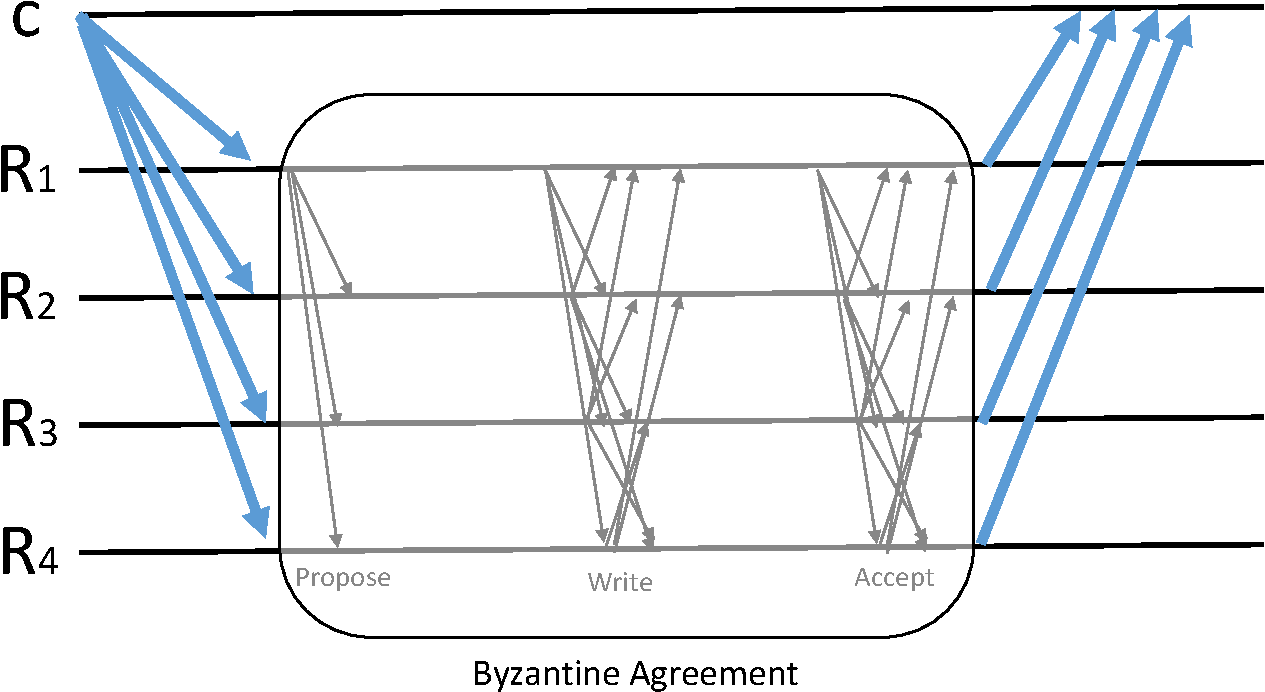
\includegraphics[width=.5\columnwidth]{images/images/bft.pdf}
\caption{Byzantine Fault Tolerance protocol overview.}
\label{fig:bft}
\end{center}
\end{figure}

Although \gls{bft} protocols provide safety to a bound of $f$ faulty nodes, with sufficient time $T$ an adversary eventually compromises $f+1$ nodes.
Then, additional mechanisms are needed to clean the faulty state (e.g., from time to time the nodes are recovered~\cite{Castro:2002}).
However, if a recovered node remains vulnerable to the same attack, the time to compromise $f+1$ becomes smaller as the attacker already knows how to exploit its vulnerabilities.
For this reason, several authors built their models assuming that the nodes fail independently due to some mechanism that provides failure independence (e.g.,~\cite{Castro:2002,Veronese:2013,Sousa:2010}).


\section{Problem Statement}
\label{sec:problemstatement}
In the last twenty years of \gls{bft} replication research, few efforts were made to justify or support the assumption that nodes fail independently. 
On contrary, there were great advances on the performance (e.g.,~\cite{Kotla:2010,Aublin:2015,Behl:2015}), use of resources (e.g.,~\cite{Yin:2003,Veronese:2013,Liu:2016,Behl:2017}), and robustness (e.g.,~\cite{Amir:2011,Bessani:2014,Clement:2009b}) of \gls{bft} systems.
These works assume, either implicitly or explicitly, that replicas fail independently, relying on some orthogonal mechanism (e.g.,~\cite{Roeder:2010,Chen:1995}) to remove common weaknesses, or rule out the possibility of malicious failures from their system models.
A few works have implemented and experimented with such mechanisms~\cite{Rodrigues:2001,Roeder:2010,Amir:2011}, but in a very limited way.
Nonetheless, in practice, diversity is a fundamental building block of dependable services in avionics~\cite{Yeh:2004}, military systems~\cite{rhimes}, and even in recent blockchain platforms such as Ethereum\footnote{\url{https://www.reddit.com/r/ethereum/comments/55s085/geth_nodes_under_attack_again_we_are_actively/}} -- three essential applications of \gls{bft}. 

A few works consider the diversity of replicas as a way to achieve such failure independence, however, it is mostly taken for granted.
For example, by using memory randomization techniques~\cite{Roeder:2010} or different \glspl{os}~\cite{Rodrigues:2001,Junqueira:2005} without providing evidence for such independence. 
Moreover, it has been shown that memory randomization does not suffice to impede common failures to occurring~\cite{Snow:2013,Bittau:2014}, and that although diversity promotes fault independence to some extent, it does not avoid utterly different \glspl{os} from sharing vulnerabilities~\cite{Garcia:2014}.

Even considering an initial set of $n$ diverse replicas, supporting the fault independence assumption, long-running services need to be cleaned from possible failures and intrusions.
A few works on the proactive recovery of \gls{bft} systems~\cite{Castro:2002,Sousa:2010,Roeder:2010,Platania:2014,Distler:2011} periodically restart their replicas to clean undetected faulty states introduced by a stealth attacker. 
However, a common limitation of these works is that they assume that these weaknesses will be cleaned after the recovery.
In practice, this will not happen unless the replica changes its software (e.g., via the previously described techniques) after its recovery.



\section{Identified Problems}
We have identified a few long-standing open problems on how \gls{bft} systems handle malicious threats. 
Some of the problems are related to how \gls{bft} replicated systems handle different types of attacks, and the others (most of them) are related to evaluating, selecting, and managing
the diversity of \gls{bft} systems:

\begin{enumerate}

\item \textbf{Traffic dissemination:} 


Most generic firewall solutions suffer from two inherent problems: 
First, they have vulnerabilities as any other system, and as a consequence, they can also be the target of advanced attacks. 
For example, the \gls{nvd}~\cite{nvd} shows that there have been many security issues in commonly used firewalls. 
\gls{nvd}'s reports present the following numbers of security issues between 2010 and 2015: 157 for the Cisco Adaptive Security Appliance; 109 in Juniper Networks solutions; 29 for the Sonicwall firewall; and 24 related to iptables/netfilter. 
Common protection solutions often have been the target of malicious actions as part of a wider scale attack (e.g., anti-virus software~\cite{Chauhan:2011}, \gls{ids}~\cite{Anderson:2001} or firewalls~\cite{Kamara:2003,Surisetty:2010,cisco1,cisco2}).
Second, firewalls are typically a single point of failure, which means that when they crash, the ability of the protected system to communicate may be compromised, at least momentarily.
Therefore, ensuring the correct operation of the firewall under a wide range of failure scenarios becomes imperative.
To tolerate faults, one typically resorts to the replication of the components.

In the last decade, several important advances occurred in the development of intrusion-tolerant systems.
However, to the best of our knowledge, very few works proposed intrusion-tolerant protection devices, such as firewalls.
Performance reasons might explain this, as \gls{bft} replication protocols are usually associated with significant overheads and limited scalability.
Additionally, achieving complete transparency to the rest of the system can be challenging to reconcile with the objective of having fast message filtering under attack.


we propose a new protection system called \sieveq that mixes the firewall paradigm with a message queue service, with the goal of improving the state-of-the-art approaches under accidental failures and/or attacks.
The solution has a fault- and intrusion-tolerant architecture that applies filtering operations in two stages acting like a sieve.
The first stage, called \emph{pre-filtering}, performs lightweight checks, making it efficient to detect and discard malicious messages from external adversaries.
In particular, messages are only allowed to go through if they come from a pre-defined set of authenticated senders.
\gls{dos} traffic from external sources is immediately dropped, preventing those messages from overloading the next stage.
The second stage, named \emph{filtering}, enforces more refined application level policies, which can require the inspection of some message fields or need the enforcement of specific ordering rules.



Typical \gls{bft} protocols use one of the two following approaches to disseminate messages to the replicas: (1) traffic replicator before the replicas or (2) a leader is responsible to dessiminate the messages to the other replicas. 
The dissemination of a message to all replicas can be detrimental to the proper operation of the replicated service.
For example, a traffic replicator device (e.g., hub) can be placed at the entry of the system to transparently reproduce all messages~\cite{Sousa:2010,Roeder:2010}. 
The effect is an attack amplification caused by the replicator device.
Alternatively, a leader replica could receive the traffic and then disseminate the messages to the others~\cite{Amir:2011}.
The drawback is that the leader becomes a natural bottleneck, especially when under attack (instead of dispersing the attack load over all replicas).
%Then, new architectures can be designed to accommodate external attacks in a resourceful and resilient manner.

In \sieveq, we explore a different design for replicated protection devices, where we trade some transparency on senders and receivers for a more efficient and resilient firewall solution.
In particular, we propose an architecture in which critical services and devices can only be accessed through a message queue and implement the application-level filtering in this queue.
It is assumed that these services have a limited number of senders, which can be appropriately configured to ensure that only they are authorized to communicate through \sieveq.


\item \textbf{Finding evidence for supporting diversity:} 
The current solutions that vouch for diversity as a way to guarantee failure independence, either lack of supporting evidence, or use evidence that is limited to some extent.
Therefore, some of the results may provide false conclusions.
We identify a need for finding \emph{accurate} sources for supporting sound evidence of the benefits diversity as a dependable mechanism.

\item \textbf{Dependably manage diversity:} 
A few works use automatic and artificial diversity (e.g.,~\cite{Roeder:2010,Amir:2011}). 
However, they lack evidence to support the failure of independence through diversity. 
Moreover, some studies show that these techniques fail to provide real diversity~\cite{Snow:2013,Bittau:2014}. 
Additionally, the existent systems that implement time-triggered recoveries assume that it takes the same time to compromise each replica. 
This assumption is unrealistic, especially when the diversity of replicas is considered. 
Therefore, it is required tailored methods to evaluate the risk of a replicated system becoming compromised.


\item \textbf{Supporting diversity mechanism:}
The few works have implemented and experimented with such mechanisms~\cite{Rodrigues:2001,Roeder:2010,Amir:2011}. 
However, despite the lack of evidence for supporting the diversity claim, they lack mechanisms that can make practical \gls{bft} systems using diversity in a continuous mode operation (i.e., with recoveries).  
Thus, reducing the costs typically associated with the management of such complex systems which deemed them as practical.


\item \textbf{Untrusted (distributed) controller:}
Solutions that implement recovery mechanisms are dependent on controller components that react (i.e., reactively or proactively) to some alarm or variable to trigger a recovery.
This type of component has been assumed to be trusted for the most existent works (e.g.,~\cite{Roeder:2010,Platania:2014,Sousa:2010}).
Moreover, they can be centralized or distributed, and in the second case it is assumed that the controller nodes are synchronous, i.e., they execute as a single node. 
We have identified a few problems on designing a solution for intrusion-tolerant (distributed) controllers. 
Although some of these problems result directly from the solutions that we have built to the previous problems, the others are more generic, and then, they can solve the existent controllers' limitations.
These problems are related to the decisions that the (distributed) controller must take in a secure way, guaranteeing that a malicious controller does not damage the integrity of the system.
For example, the controller nodes need to be proactive in taking some actions without harming \gls{smr} properties.
Some of these decisions require secure distributed random number generation, or to take ``synchronous'' decisions (e.g., update a replicated database at the same time).  
Another problem that must be addressed is the way that data is stored among the controllers, which in the existent solutions is always centralized or distributed and trusted. 


\end{enumerate}


\section{Summary of the Contributions}
\label{sec:contributions}


In this thesis, we present the contributions that we propose to solve the previously enumerated problems. 



We design a new architecture to solve the \emph{dissemination problem}, and the envisioned solution applies filtering operations in two stages acting like a sieve.
We introduced a first pre-filtering stage that performs lightweight checks, making it efficient to detect and discard malicious messages from external adversaries.
This effort resulted in a \gls{bft} system named \sieveq, that mixes the firewall paradigm with a message queue service, with the goal of improving the state-of-the-art approaches under accidental failures and/or attacks. 
\sieveq was experimentally evaluated in different scenarios, and the results show that it is much more resilient to \gls{dos} attacks and various kinds of intrusions than existing replicated-firewall approaches.
The contributions of this work resulted in the following publications:

\begin{enumerate}
\item[1.] \emph{An Intrusion-Tolerant Firewall Design for Protecting SIEM Systems, Miguel Garcia, Nuno Neves, Alysson Bessani, in the Workshop on Systems Resilience in conjunction with the IEEE/IFIP International Conference on Dependable Systems and Networks, 2013}~\cite{Garcia:2013}.

\item[2.] \emph{\sieveq: A Layered BFT Protection System for Critical Services, Miguel Garcia, Nuno Neves, and Alysson Bessani, in IEEE Transactions on Dependable and Secure Computing, 2018}~\cite{Garcia:2016}.
\end{enumerate}


We address the problems of \emph{finding evidence for supporting diversity}, \emph{manage diversity in a dependable way}, and \emph{supporting diversity mechanism} in the thesis main contribution.
We use different \gls{osint} data sources to build a complete knowledge base about the possible vulnerabilities, exploits, and patches related to the systems of interest. 
Moreover, this data is used to create clusters of similar vulnerabilities, which potentially can be affected by (variations of) the same exploit. 
These clusters and the other collected data are used to assess the risk of the \gls{bft} system becoming compromised due to common vulnerabilities.
Once the risk increases, the system replaces the potentially vulnerable replica by another one, to maximize the failure independence of the replicated service.
The solution continuously collects data from the online sources and monitors the risk of the \gls{bft} in such a way that removes the human from the loop.
We developed these contributions in a solution named \system, and it is the first system that manages \gls{bft} replicated systems (e.g., \sieveq) in a dependable and automatic way.
\system experimental evaluation shows that its strategy reduces the number of executions where the system becomes compromised and that our prototype supports the execution of full-fledged \gls{bft} systems in diverse configurations with 17 \gls{os} versions, reaching a performance close to a homogeneous bare metal setup. 


The contributions of this work resulted in the following publications:

\begin{enumerate}

\item[3] \emph{Towards an Execution Environment for Intrusion-Tolerant Systems, Miguel Garcia, Alysson Bessani, and Nuno Neves, Poster session in the European Conference on Computer Systems (EuroSys), 2016}~\cite{Garcia:2016b}.


\item[4.] \emph{\system: Automatic Management of Diversity in BFT Systems, Miguel Garcia, Alysson Bessani, and Nuno Neves}~\cite{}.

\end{enumerate}


In the previous contribution, we presented a controller that was logically-centralized. \side{RE-DO}
In the following publication we present \controller, a generic \gls{bft}-controller for \gls{bft} systems that eliminates some of \system' assumptions:


\begin{enumerate}

\item[5.] \emph{\controller Miguel Garcia, Alysson Bessani, and Nuno Neves}~\cite{}.

\end{enumerate}

We summarize our findings in the following thesis statement:


\vspace{2mm}
\fbox{ \begin{minipage}{35em}
%\begin{center}
\emph{
It is possible to build dependable BFT replicated systems by minimizing the number of replicas' common vulnerabilities through software's diversity.
Additionally, it is possible to continuously manage these systems while monitoring OSINT data and deciding when replicas should be diversified and deploying the most dependable configurations.
}
%\end{center}
\end{minipage}
}


Although these are not directly related to this thesis, we present the following publications:

The results achieved during the MSc thesis encouraged us to extend the work on \gls{ots} \glspl{os} common vulnerabilities.
In this extension, we devised three manual strategies for selecting diverse software components to minimize the incidence of common vulnerabilities in replicated systems.
Moreover, we observed that using different \gls{os} releases of the same \gls{os} are enough to warrant its adoption as a more straightforward, less complicated, more manageable configuration for replicated systems.

\begin{enumerate}
\item[6.] \emph{Analysis of operating system diversity for intrusion tolerance, Miguel Garcia, Alysson Bessani, Ilir Gashi Nuno Neves, and Rafael Obelheiro, in Software: Practice and Experience, 2014}~\cite{Garcia:2014}.
\end{enumerate}


The following work describes a \gls{scada} system enhanced with \gls{bft} techniques.
We document the challenges of building such system from a ``traditional'' non-\gls{bft} solution.
This effort resulted in a prototype that integrates the Eclipse NeoSCADA and the BFT-SMaRt open-source projects.
This solution could be managed by \system.

\begin{enumerate}

\item[7.] \emph{On the Challenges of Building a BFT SCADA, Andr\'{e} Nogueira, Miguel Garcia, Alysson Bessani, and Nuno Neves, in Proceedings of the International Conference on Dependable Systems and Networks, 2018 }~\cite{Nogueira:2018}.
\end{enumerate}



%\emph{It is possible to manage the risk of \gls{bft} systems by analyzing updated online data sources to make decisions while guaranteeing failure independence through automatic diversity rejuvenations with minor performance impacts?}
Table~\ref{tab:map} presents how we map the different identified problems into publications, chapters, and solution tools.


\begin{table}[h]
\begin{center}
\begin{tabular}{ c  c c c }\hline
\textbf{Identified Problems} & \textbf{Publication}  & \textbf{Chapter} & \textbf{Solution tool}  \\ \hline			
1. & (2), (3) &  & \sieveq\\ \hline			
2. 3. 4. & (1), (4), (5)  & &  \system  \\ \hline			
5. & (6) &  & \controller \\  \hline			
\end{tabular}
\caption{Overview of the mapping of open problems, published contributions, and chapters.}
\label{tab:map}
\end{center}
\end{table}



\section{Document Structure}
\label{sec:documentstructure}
%The rest of the document is organized as follows:
%In Chapter~\ref{chap:literaturereview} we make a literature review of the most relevant and related works to this thesis contributions.
%In Chapter~\ref{chap:overview} we present the system model and preliminary details that are relevant for the rest of the thesis.
%The first contribution, \sieveq, is presented in Chapter~\ref{chap:sieveq}.
%The second contribution, \system, is presented in Chapter~\ref{chap:lazarus}.
%The last contribution, \controller, is presented in Chapter~\ref{chap:controler}.
%Then, we present the evaluation experiments for both \sieveq and \system contributions, in Chapter~\ref{chap:sieveqevaluation} and in Chapter~\ref{chap:lazarusevaluation}, respectively.
%Finally, we conclude the thesis in Chapter~\ref{chap:conclusion} with a summary of the its achievements and with a discussion on the open avenues for future work resulting from the thesis.


